\section{eo\-Easy\-EA$<$ EOT $>$ Class Template Reference}
\label{classeo_easy_e_a}\index{eoEasyEA@{eoEasyEA}}
An easy-to-use evolutionary algorithm; you can use any chromosome, and any selection transformation, merging and evaluation algorithms; you can even change in runtime parameters of those sub-algorithms.  


{\tt \#include $<$eo\-Easy\-EA.h$>$}

Inheritance diagram for eo\-Easy\-EA$<$ EOT $>$::\begin{figure}[H]
\begin{center}
\leavevmode
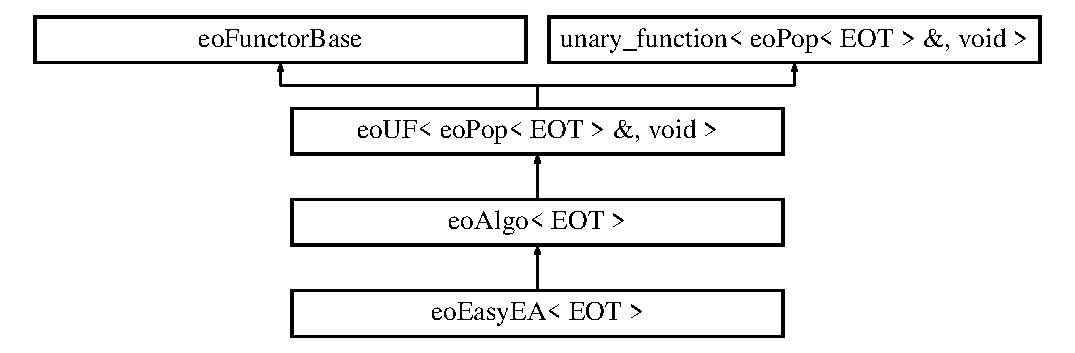
\includegraphics[height=4cm]{classeo_easy_e_a}
\end{center}
\end{figure}
\subsection*{Public Member Functions}
\begin{CompactItemize}
\item 
{\bf eo\-Easy\-EA} ({\bf eo\-Continue}$<$ {\bf EOT} $>$ \&\_\-continuator, {\bf eo\-Eval\-Func}$<$ {\bf EOT} $>$ \&\_\-eval, {\bf eo\-Breed}$<$ {\bf EOT} $>$ \&\_\-breed, {\bf eo\-Replacement}$<$ {\bf EOT} $>$ \&\_\-replace)\label{classeo_easy_e_a_a0}

\begin{CompactList}\small\item\em Ctor taking a breed and merge. \item\end{CompactList}\item 
{\bf eo\-Easy\-EA} ({\bf eo\-Continue}$<$ {\bf EOT} $>$ \&\_\-continuator, {\bf eo\-Pop\-Eval\-Func}$<$ {\bf EOT} $>$ \&\_\-eval, {\bf eo\-Breed}$<$ {\bf EOT} $>$ \&\_\-breed, {\bf eo\-Replacement}$<$ {\bf EOT} $>$ \&\_\-replace)\label{classeo_easy_e_a_a1}

\begin{CompactList}\small\item\em NEW Ctor taking a breed and merge and an eo\-Pop\-Eval. \item\end{CompactList}\item 
{\bf eo\-Easy\-EA} ({\bf eo\-Continue}$<$ {\bf EOT} $>$ \&\_\-continuator, {\bf eo\-Eval\-Func}$<$ {\bf EOT} $>$ \&\_\-eval, {\bf eo\-Breed}$<$ {\bf EOT} $>$ \&\_\-breed, {\bf eo\-Merge}$<$ {\bf EOT} $>$ \&\_\-merge, {\bf eo\-Reduce}$<$ {\bf EOT} $>$ \&\_\-reduce)\label{classeo_easy_e_a_a2}

\begin{CompactList}\small\item\em Ctor {\bf eo\-Breed}{\rm (p.\,\pageref{classeo_breed})}, {\bf eo\-Merge}{\rm (p.\,\pageref{classeo_merge})} and {\bf eo\-Reduce}{\rm (p.\,\pageref{classeo_reduce})}. \item\end{CompactList}\item 
{\bf eo\-Easy\-EA} ({\bf eo\-Continue}$<$ {\bf EOT} $>$ \&\_\-continuator, {\bf eo\-Eval\-Func}$<$ {\bf EOT} $>$ \&\_\-eval, {\bf eo\-Select}$<$ {\bf EOT} $>$ \&\_\-select, {\bf eo\-Transform}$<$ {\bf EOT} $>$ \&\_\-transform, {\bf eo\-Replacement}$<$ {\bf EOT} $>$ \&\_\-replace)\label{classeo_easy_e_a_a3}

\begin{CompactList}\small\item\em Ctor {\bf eo\-Select}{\rm (p.\,\pageref{classeo_select})}, {\bf eo\-Transform}{\rm (p.\,\pageref{classeo_transform})}, and {\bf eo\-Replacement}{\rm (p.\,\pageref{classeo_replacement})}. \item\end{CompactList}\item 
{\bf eo\-Easy\-EA} ({\bf eo\-Continue}$<$ {\bf EOT} $>$ \&\_\-continuator, {\bf eo\-Eval\-Func}$<$ {\bf EOT} $>$ \&\_\-eval, {\bf eo\-Select}$<$ {\bf EOT} $>$ \&\_\-select, {\bf eo\-Transform}$<$ {\bf EOT} $>$ \&\_\-transform, {\bf eo\-Merge}$<$ {\bf EOT} $>$ \&\_\-merge, {\bf eo\-Reduce}$<$ {\bf EOT} $>$ \&\_\-reduce)\label{classeo_easy_e_a_a4}

\begin{CompactList}\small\item\em Ctor {\bf eo\-Select}{\rm (p.\,\pageref{classeo_select})}, {\bf eo\-Transform}{\rm (p.\,\pageref{classeo_transform})}, {\bf eo\-Merge}{\rm (p.\,\pageref{classeo_merge})} and {\bf eo\-Reduce}{\rm (p.\,\pageref{classeo_reduce})}. \item\end{CompactList}\item 
virtual void {\bf operator()} ({\bf eo\-Pop}$<$ {\bf EOT} $>$ \&\_\-pop)\label{classeo_easy_e_a_a5}

\begin{CompactList}\small\item\em Apply a few generation of evolution to the population. \item\end{CompactList}\end{CompactItemize}
\subsection*{Protected Attributes}
\begin{CompactItemize}
\item 
eo\-Easy\-EA::eo\-Dummy\-Select {\bf dummy\-Select}\label{classeo_easy_e_a_p0}

\item 
eo\-Easy\-EA::eo\-Dummy\-Transform {\bf dummy\-Transform}\label{classeo_easy_e_a_p1}

\item 
eo\-Easy\-EA::eo\-Dummy\-Eval {\bf dummy\-Eval}\label{classeo_easy_e_a_p2}

\item 
{\bf eo\-Continue}$<$ {\bf EOT} $>$ \& {\bf continuator}\label{classeo_easy_e_a_p3}

\item 
{\bf eo\-Eval\-Func}$<$ {\bf EOT} $>$ \& {\bf eval}\label{classeo_easy_e_a_p4}

\item 
{\bf eo\-Pop\-Loop\-Eval}$<$ {\bf EOT} $>$ {\bf loop\-Eval}\label{classeo_easy_e_a_p5}

\item 
{\bf eo\-Pop\-Eval\-Func}$<$ {\bf EOT} $>$ \& {\bf pop\-Eval}\label{classeo_easy_e_a_p6}

\item 
{\bf eo\-Select\-Transform}$<$ {\bf EOT} $>$ {\bf select\-Transform}\label{classeo_easy_e_a_p7}

\item 
{\bf eo\-Breed}$<$ {\bf EOT} $>$ \& {\bf breed}\label{classeo_easy_e_a_p8}

\item 
{\bf eo\-No\-Elitism}$<$ {\bf EOT} $>$ {\bf dummy\-Merge}\label{classeo_easy_e_a_p9}

\item 
{\bf eo\-Truncate}$<$ {\bf EOT} $>$ {\bf dummy\-Reduce}\label{classeo_easy_e_a_p10}

\item 
{\bf eo\-Merge\-Reduce}$<$ {\bf EOT} $>$ {\bf merge\-Reduce}\label{classeo_easy_e_a_p11}

\item 
{\bf eo\-Replacement}$<$ {\bf EOT} $>$ \& {\bf replace}\label{classeo_easy_e_a_p12}

\end{CompactItemize}
\subsection*{Friends}
\begin{CompactItemize}
\item 
class {\bf eo\-Islands\-Easy\-EA$<$EOT$>$}\label{classeo_easy_e_a_n0}

\item 
class {\bf eo\-Dist\-Eval\-Easy\-EA$<$EOT$>$}\label{classeo_easy_e_a_n1}

\end{CompactItemize}


\subsection{Detailed Description}
\subsubsection*{template$<$class EOT$>$ class eo\-Easy\-EA$<$ EOT $>$}

An easy-to-use evolutionary algorithm; you can use any chromosome, and any selection transformation, merging and evaluation algorithms; you can even change in runtime parameters of those sub-algorithms. 

Change (MS, July 3. 2001): Replaced the {\bf eo\-Eval\-Func}{\rm (p.\,\pageref{classeo_eval_func})} by an {\bf eo\-Pop\-Eval\-Func}{\rm (p.\,\pageref{classeo_pop_eval_func})}: this immediately allows many useful constructs, such as co-evolution (e.g. game players), parisian approach (the solution to the problem is the whole population) or simple distribution of evaluations on a cluster. In case an {\bf eo\-Eval\-Func}{\rm (p.\,\pageref{classeo_eval_func})} is passed, it is embedded on an {\bf eo\-Pop\-Loop\-Eval}{\rm (p.\,\pageref{classeo_pop_loop_eval})} This makes things a little uglier (required an additional \char`\"{}dummy\char`\"{} member

Note: it looks ugly only because we wanted to authorize many different constructors. Please only look at the operator() and there shall be light 



Definition at line 63 of file eo\-Easy\-EA.h.

The documentation for this class was generated from the following file:\begin{CompactItemize}
\item 
eo\-Easy\-EA.h\end{CompactItemize}
